\subsection{Transforms}
\label{sec:transforms}

The transforms \ac{API} was designed to be similar to the PyTorch
\linebreak
\texttt{torchvision.transforms} module.
%
TorchIO includes augmentations such as
random affine transformation (\cref{fig:raffine})
or random blur (\cref{fig:rblur}),
but they are implemented using medical imaging
libraries \cite{lowekamp_design_2013,brett_nipynibabel_2020}
to take into account specific properties of medical images,
namely their size, resolution, location, and orientation (see \cref{sec:metadata}).
%
\cref{tab:transforms} shows transforms implemented in TorchIO \torchioversion
and their main corresponding library dependencies.


\begin{table}[ht]
    \caption{
        Transforms included in TorchIO \torchioversion.
        Logos indicate the main library used to process the images.
        \protect\logo{nipy}:~NiBabel \cite{brett_nipynibabel_2020};
        \protect\logo{itk}:~SimpleITK \cite{lowekamp_design_2013};
        \protect\logo{numpy}:~NumPy \cite{van_der_walt_numpy_2011};
        \protect\logo{pytorch}:~PyTorch \cite{paszke_pytorch_2019}.
    }
    \footnotesize
    \begin{center}
        \begin{tabular}{c||c|c}
                                                    & \textbf{Spatial}                      & \textbf{Intensity}                                                      \\
            \hline
            \hline
            \multirow{5}{*}{\textbf{Preprocessing}} & \trsfl{ToCanonical}{nipy}             &                                                                         \\
                                                    & \trsfl{Resample}{itk}                 & \trsfl{HistogramStandardization}{numpy} \cite{nyul_standardizing_1999} \\
                                                    & \trsfl{Crop}{itk}                     & \trsfl{RescaleIntensity}{numpy}                                         \\
                                                    & \trsfl{Pad}{itk}                      & \trsfl{ZNormalization}{pytorch}                                         \\
                                                    & \trsfl{CropOrPad}{itk}                &                                                                         \\
            \hline
            \multirow{7}{*}{\textbf{Augmentation}}  &                                       & \trsfl{RandomMotion}{numpy} \cite{shaw_mri_2019}                       \\
                                                    &                                       & \trsfl{RandomBiasField}{numpy} \cite{sudre_longitudinal_2017}          \\
                                                    &                                       & \trsfl{RandomGhosting}{numpy}                                           \\
                                                    & \trsfl{RandomAffine}{itk}             & \trsfl{RandomSpike}{numpy} \cite{shaw_heteroscedastic_2020}            \\
                                                    & \trsfl{RandomElasticDeformation}{itk} & \trsfl{RandomBlur}{numpy}                                               \\
                                                    & \trsfl{RandomFlip}{pytorch}           & \trsfl{RandomGamma}{pytorch}                                            \\
                                                    &                                       & \trsfl{RandomNoise}{pytorch}                                            \\
                                                    &                                       & \trsfl{RandomSwap}{pytorch} \cite{chen_self-supervised_2019}           \\
                                                    &                                       & \trsfl{RandomLabelsToImage}{pytorch} \cite{billot_learning_2020}       \\
                                                    &                                       & \trsfl{RandomAnisotropy}{itk} \cite{billot_partial_2020}               \\
        \end{tabular}
    \end{center}
    \label{tab:transforms}
\end{table}



Transforms are designed to be flexible regarding input and output types.
%
Following a duck typing approach,
they can take as input
PyTorch tensors,
SimpleITK images,
NumPy arrays,
Pillow images,
Python dictionaries,
and instances of
\texttt{Subject}
and \texttt{Image},
and will return an output of the same type.


TorchIO transforms can be classified into either spatial and intensity transforms,
or preprocessing and augmentation transforms (\cref{tab:transforms}).
%
All are subclasses of the \texttt{Transform} base class.
%
Spatial transforms and intensity transforms are related to the
\texttt{SpatialTransform} and \texttt{IntensityTransform} classes, respectively.
%
Transforms whose parameters are randomly chosen are subclasses of \texttt{RandomTransform}.


Instances of \texttt{SpatialTransform} typically modify the image bounds or spacing, and often need
to resample the image using interpolation.
%
They are applied to all image types.
%
Instances of \texttt{IntensityTransform} do not modify the position of voxels, only their values,
and they are only applied to instances of \texttt{ScalarImage}.
%
For example, if a \texttt{RandomNoise} transform
(which is a subclass of
\texttt{IntensityTransform})
receives as input
a \texttt{Subject} with a \texttt{ScalarImage} representing
a \ac{CT} scan and a \texttt{LabelMap} representing a segmentation,
it will add noise to only the \ac{CT} scan.
%
On the other hand, if a \texttt{RandomAffine} transform
(which is a subclass of \texttt{SpatialTransform}) receives the same input,
the same affine transformation will be applied to both images,
with nearest-neighbor interpolation always used to interpolate
\texttt{LabelMap} objects.

\comment{% Rachel says this might not be necessary
Preprocessing transforms are typically applied to normalize images during
training and inference, whereas augmentation transforms
are random operations applied during training to artificially increase the
size of the training dataset \cite{shorten_survey_2019}.
}


\subsubsection{Preprocessing}

Preprocessing transforms are necessary to ensure
spatial and intensity uniformity of training instances.


Spatial preprocessing is important as \acp{CNN} do not generally take into
account metadata related to medical images (see \cref{sec:metadata}),
therefore it is necessary to ensure that voxels across images have
similar spatial location and relationships before training.
%
Spatial preprocessing transforms typically used in medical imaging include
resampling (e.g., to make voxel spacing isotropic for all training samples)
and reorientation (e.g., to orient all training samples in
the same way).
%
For example, the \texttt{Resample} transform can be used to fix the issue
presented in \cref{fig:metadata}.


Intensity normalization is generally beneficial
for optimization of neural networks.
%
TorchIO provides intensity
normalization techniques including min-max scaling or
standardization\footnote{In this context,
standardization refers to correcting voxel intensity values
to have zero mean and unit variance.},
which are computed using pure PyTorch.
%
A binary image, such as a mask representing the foreground
or structures of interest,
can be used to define the set of voxels to be taken into account
when computing statistics for intensity normalization.
%
We also provide a method for \ac{MRI} histogram
standardization \cite{nyul_new_2000}, computed using NumPy,
which may be used to overcome the differences
in intensity distributions between images acquired using
different scanners or sequences.

\begin{figure}
    \centering
    \captionsetup[subfigure]{aboveskip=0pt, belowskip=3pt}

    \begin{subfigure}{0.45\textwidth}
        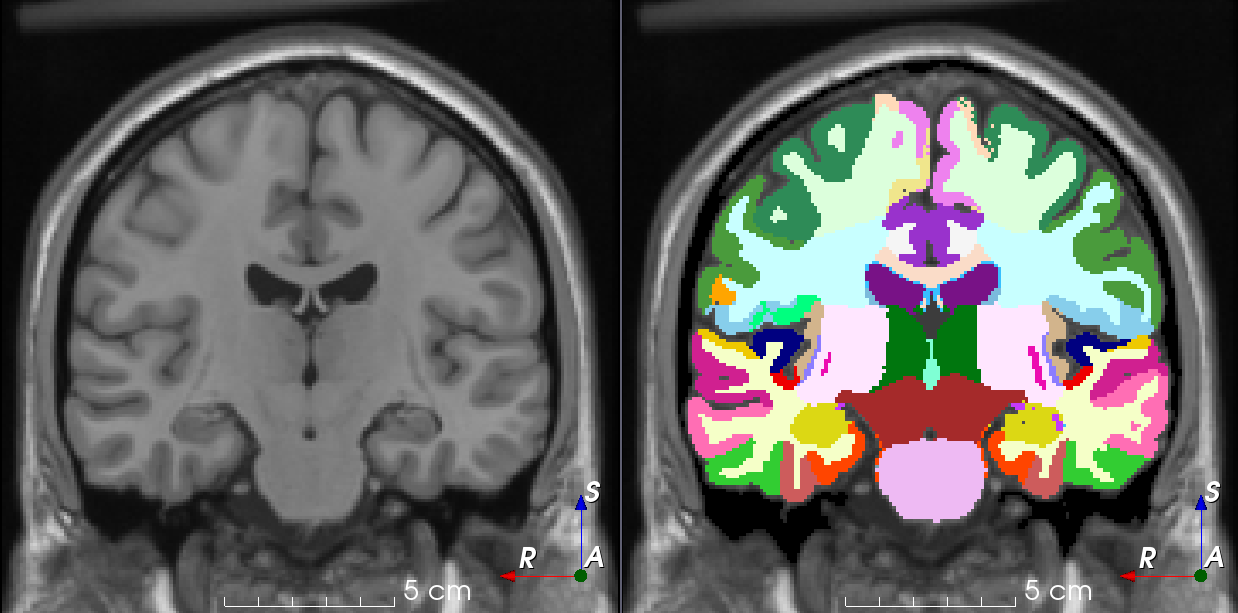
\includegraphics[width=0.98\linewidth]{colin27_t1_tal_lin_mri}
        \caption{Original image and segmentation}
        \label{fig:original}
    \end{subfigure}%
    \hspace{2em}%
    \begin{subfigure}{0.45\textwidth}
        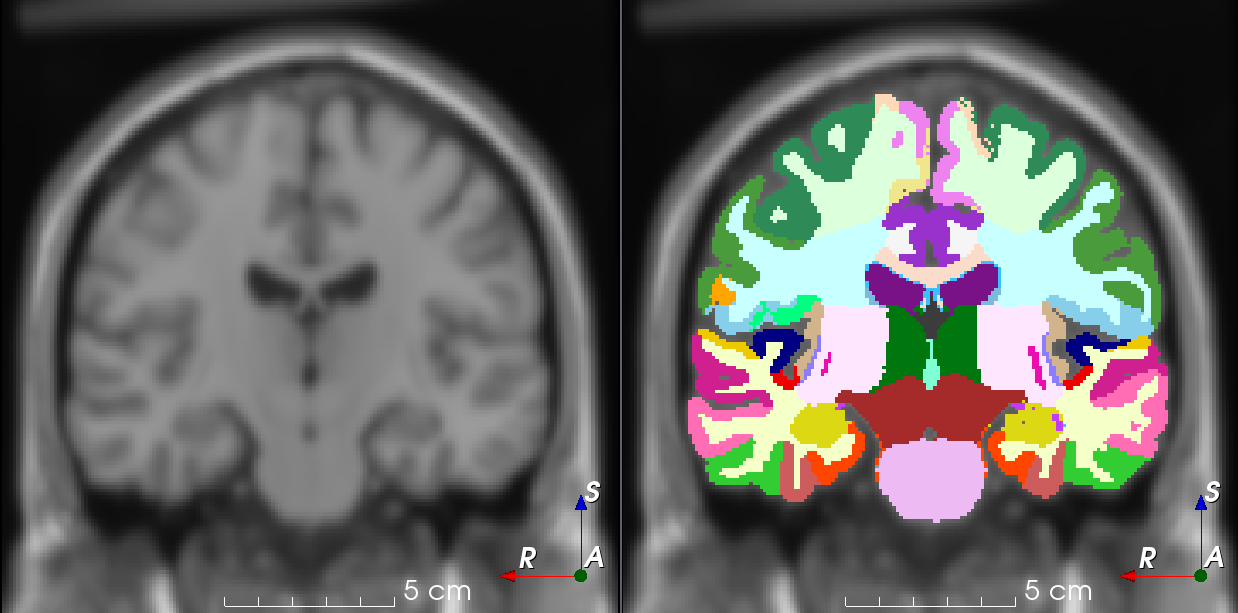
\includegraphics[width=0.98\linewidth]{0_RandomBlur_mri}
        \caption{Random blur}
        \label{fig:rblur}
    \end{subfigure}

    \begin{subfigure}{0.45\textwidth}
        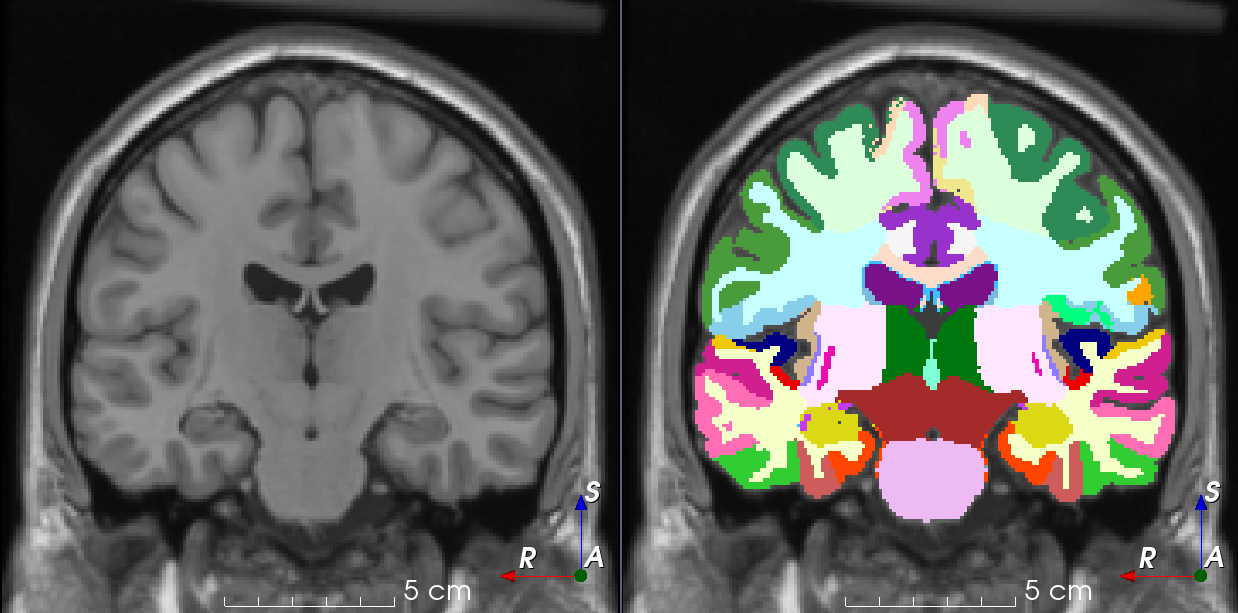
\includegraphics[width=0.98\linewidth]{1_RandomFlip_mri}
        \caption{Random flip}
        \label{fig:rflip}
    \end{subfigure}%
    \hspace{2em}%
    \begin{subfigure}{0.45\textwidth}
        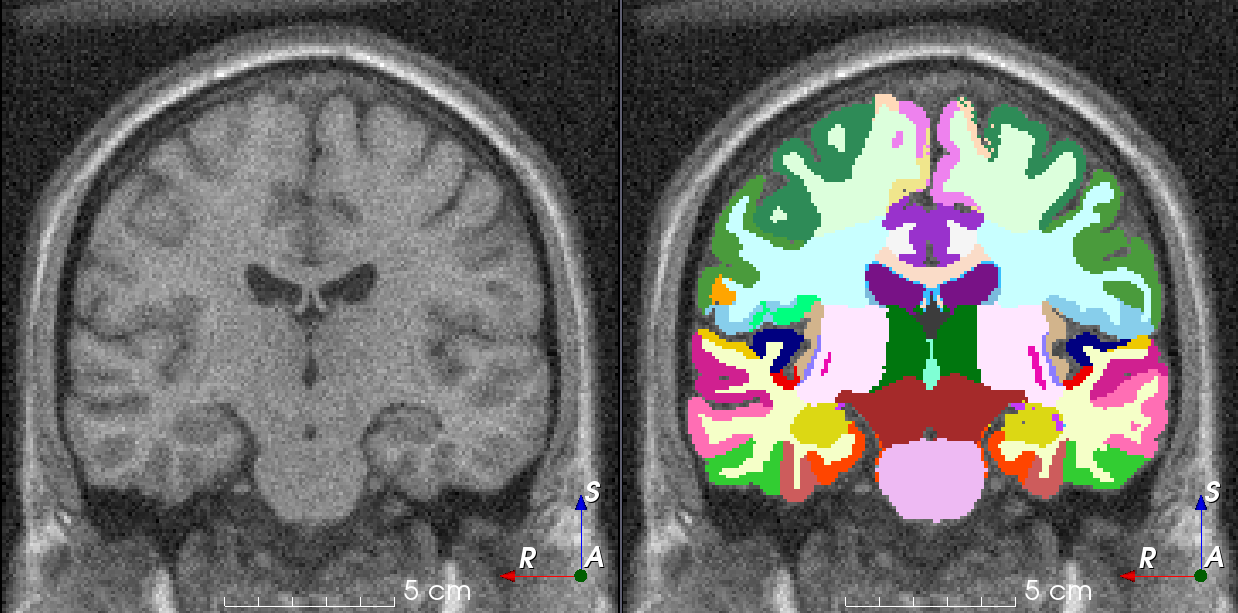
\includegraphics[width=0.98\linewidth]{2_Compose_mri}
        \caption{Random noise}
        \label{fig:rnoise}
    \end{subfigure}

    \begin{subfigure}{0.45\textwidth}
        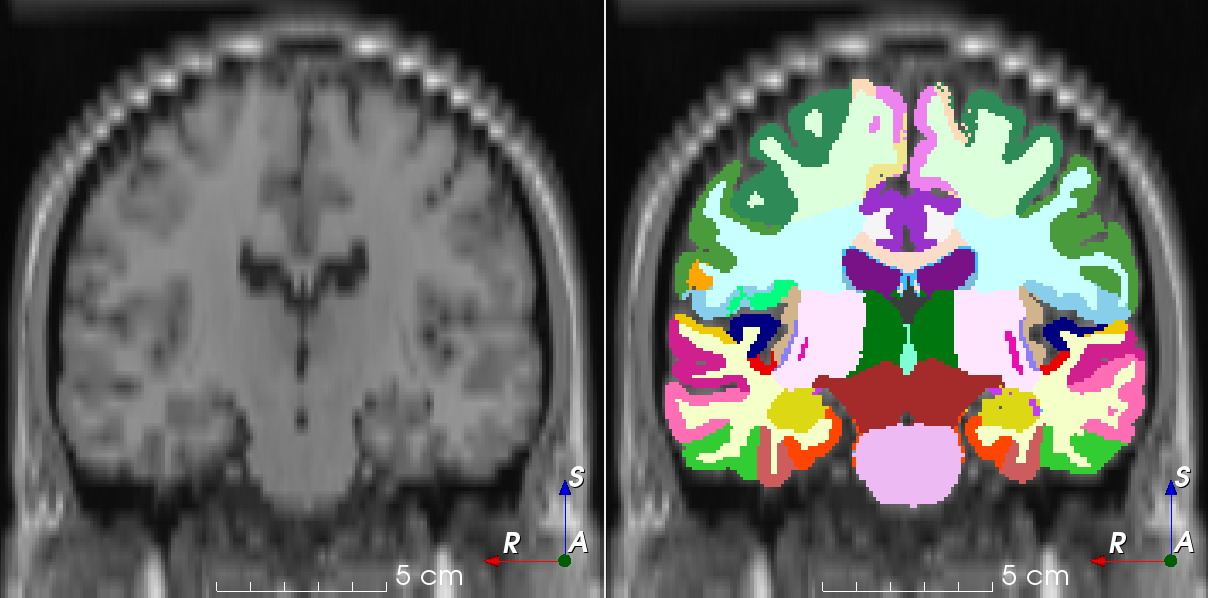
\includegraphics[width=0.98\linewidth]{0_RandomAnisotropy_mri}
        \caption{Random anisotropy}
        \label{fig:raffine}
    \end{subfigure}%
    \hspace{2em}%
    \begin{subfigure}{0.45\textwidth}
        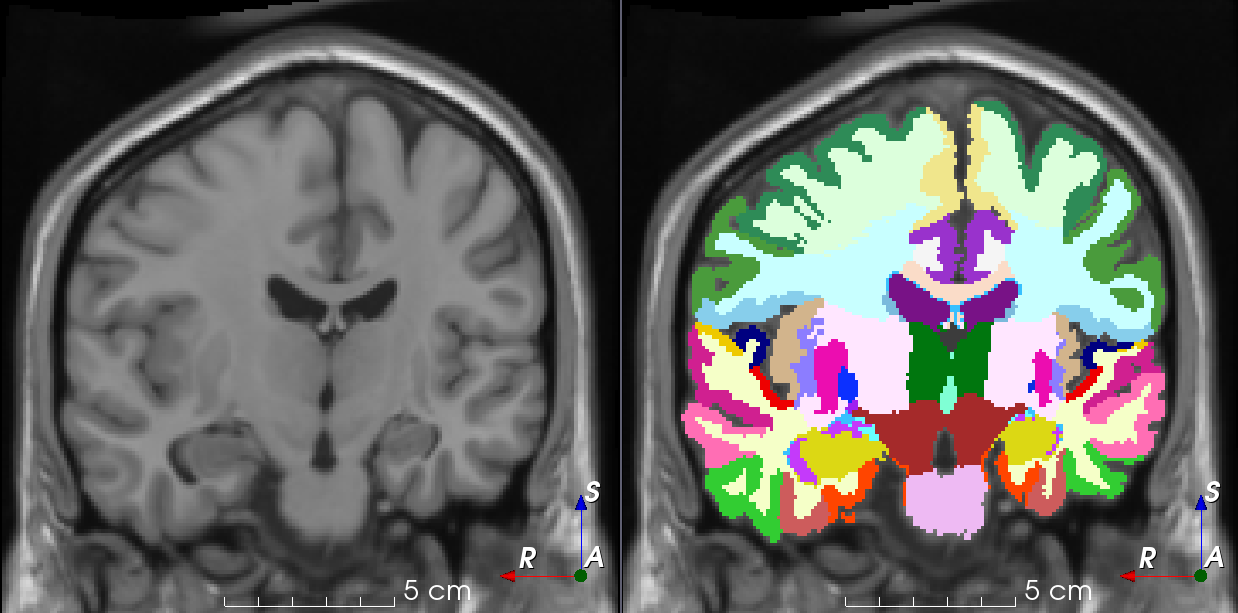
\includegraphics[width=0.98\linewidth]{4_RandomElasticDeformation_mri}
        \caption{Random elastic transformation}
        \label{fig:relastic}
    \end{subfigure}

    \begin{subfigure}{0.45\textwidth}
        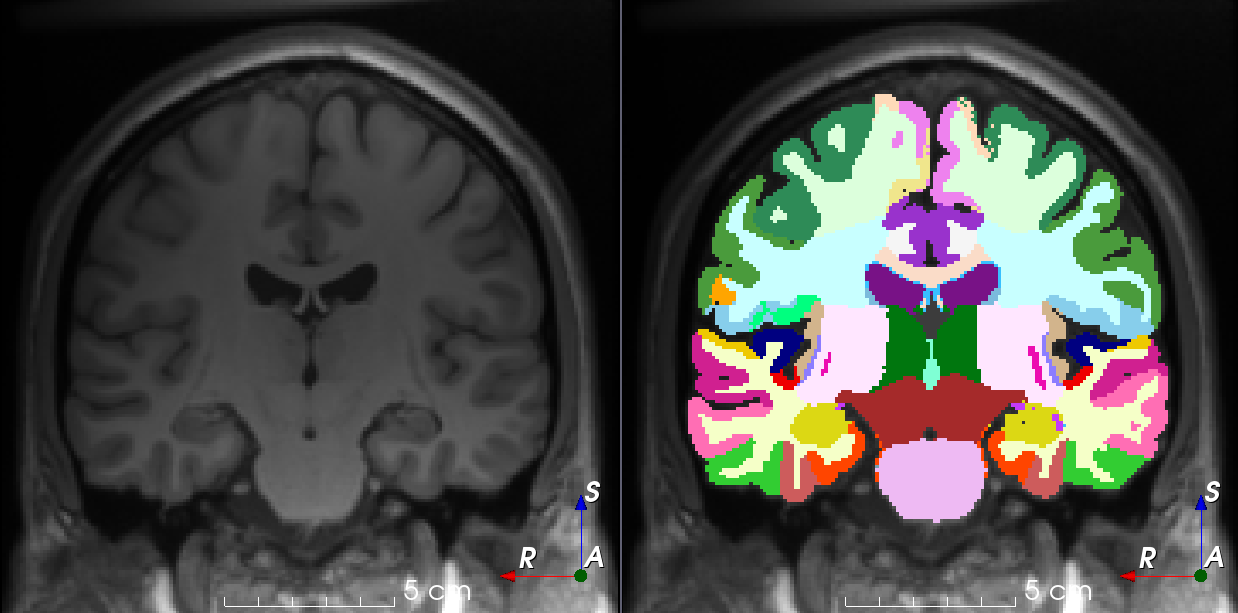
\includegraphics[width=0.98\linewidth]{5_RandomBiasField_mri}
        \caption{Random bias field artifact}
        \label{fig:rbias}
    \end{subfigure}%
    \hspace{2em}%
    \begin{subfigure}{0.45\textwidth}
        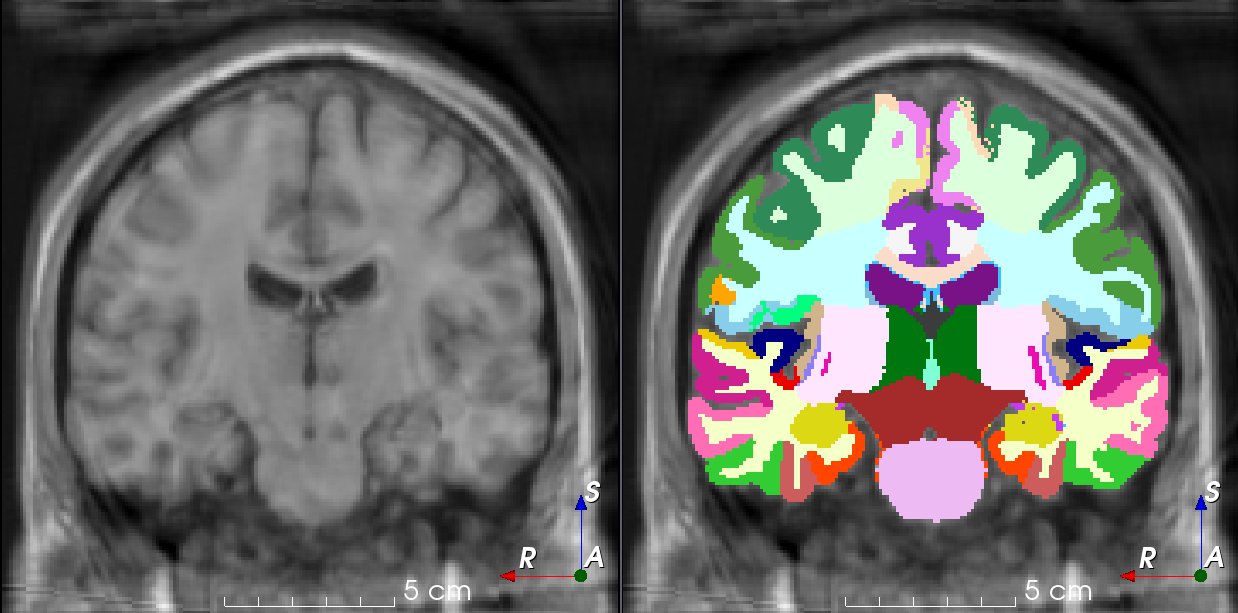
\includegraphics[width=0.98\linewidth]{6_RandomMotion_mri}
        \caption{Random motion artifact}
        \label{fig:rmotion}
    \end{subfigure}

    \begin{subfigure}{0.45\textwidth}
        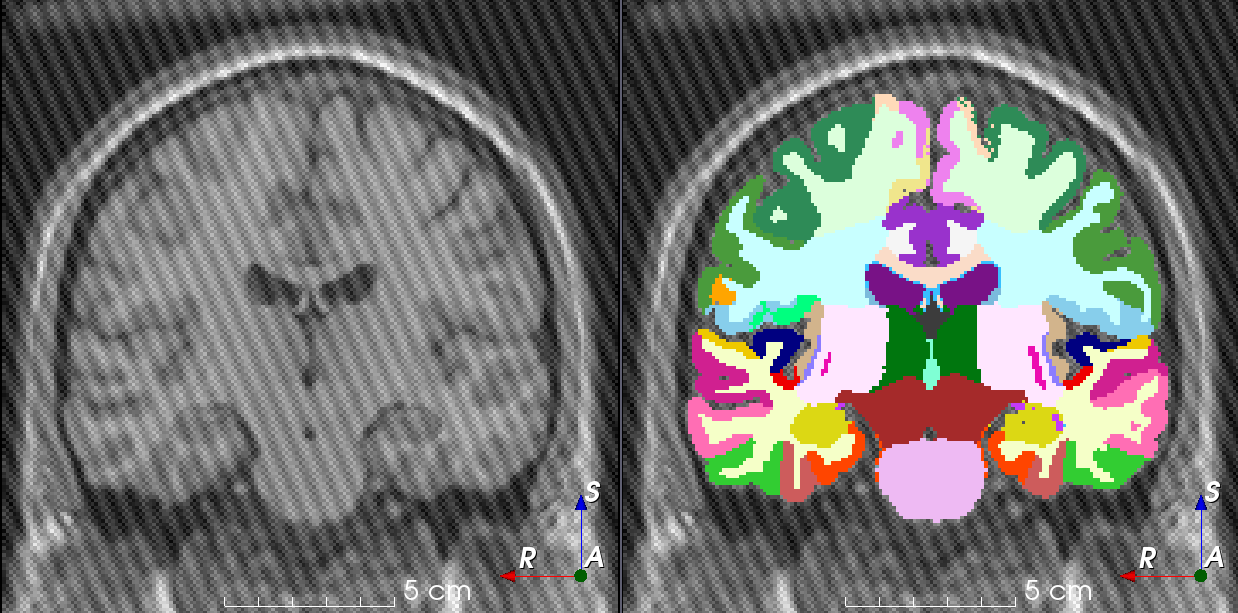
\includegraphics[width=0.98\linewidth]{7_RandomSpike_mri}
        \caption{Random spike artifact}
        \label{fig:rspike}
    \end{subfigure}%
    \hspace{2em}%
    \begin{subfigure}{0.45\textwidth}
        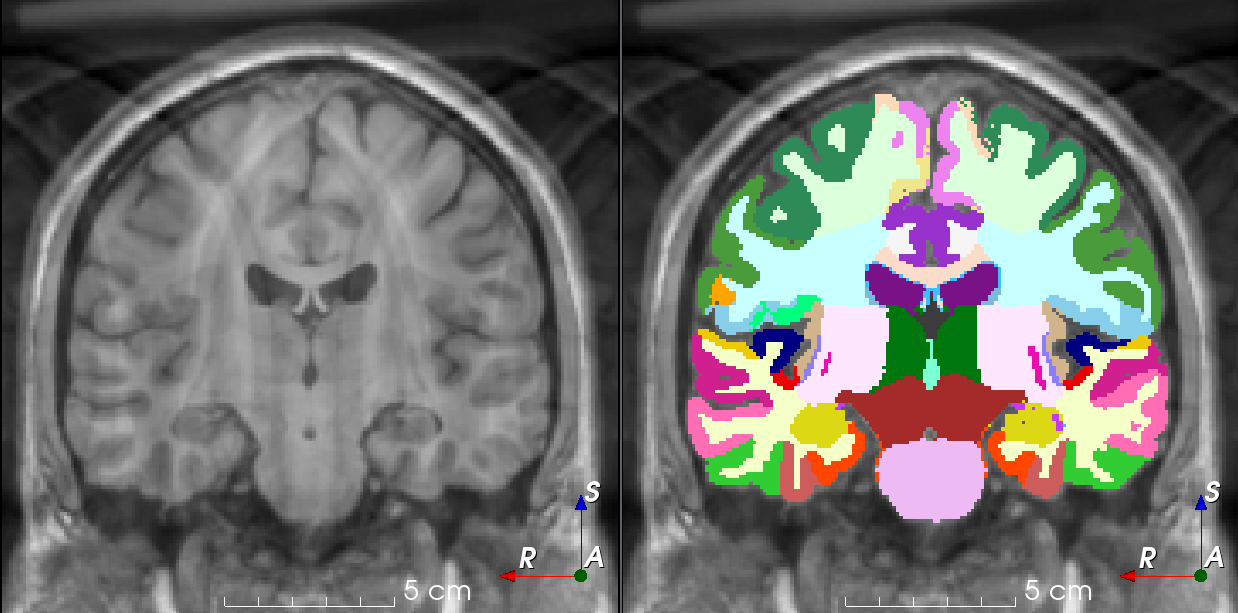
\includegraphics[width=0.98\linewidth]{8_RandomGhosting_mri}
        \caption{Random ghosting artifact}
        \label{fig:rghost}
    \end{subfigure}

    \caption{%
        A selection of data augmentation techniques
        available in TorchIO \torchioversion.
        Each example is presented as a pair of images composed of the
        transformed image and a corresponding transformed label map.
        Note that all screenshots are from a 2D coronal slice
        of the transformed 3D images.
        The \ac{MRI} corresponds to the \ac{MNI} Colin 27
        average brain \cite{holmes_enhancement_1998}, which can
        be downloaded using \texttt{torchio.datasets.Colin27}.
        Label maps were generated using an automated brain parcellation
        algorithm \cite{cardoso_geodesic_2015}.
    }
    \label{fig:augmentations}
\end{figure}

\acreset{mni}  % we want to describe it in the text as well

\subsubsection{Augmentation}

TorchIO includes spatial augmentation transforms such as random flipping using
PyTorch and random affine and elastic deformation transforms using SimpleITK.
%
Intensity augmentation transforms include
random Gaussian blur using a SimpleITK filter (\cref{fig:rblur})
and addition of random Gaussian noise using pure PyTorch (\cref{fig:rnoise}).
% %
% \Cref{fig:augmentations} shows examples of augmentation transforms
% implemented in TorchIO.
All augmentation transforms are subclasses of \texttt{RandomTransform}.


Although current domain-specific data augmentation transforms available
in TorchIO are mostly related to \ac{MRI},
we encourage users to contribute physics-based data augmentation
techniques for \ac{US} or \ac{CT} \cite{omigbodun_effects_2019}.


We provide several \ac{MRI}-specific augmentation transforms
related to $k$-space, which are described below.
%
An MR image is usually reconstructed as the magnitude
of the inverse Fourier transform of the $k$-space signal, which is populated with
the signals generated by the sample
as a response to a radio-frequency electromagnetic pulse.
%
These signals are modulated using coils that create gradients of the magnetic
field inside the scanner.
%
Artifacts are created by using $k$-space transforms to perturb the Fourier space
and generate corresponding intensity artifacts in image space.
%
The forward and inverse Fourier transforms are computed using the
\ac{FFT} algorithm implemented in NumPy.


\paragraph{Random $k$-space spike artifact}

Gradients applied at a very high duty cycle may produce bad
data points, or noise spikes, in $k$-space \cite{zhuo_mr_2006}.
%
These points in $k$-space generate a spike artifact,
also known as Herringbone, crisscross or corduroy artifact,
which manifests as uniformly-separated stripes in image space,
as shown in \cref{fig:rspike}.
%
This type of data augmentation has recently been used to estimate uncertainty
through a heteroscedastic noise model \cite{shaw_heteroscedastic_2020}.


\paragraph{Random $k$-space motion artifact}

The $k$-space is often populated line by line,
and the sample in the scanner is assumed to remain static.
%
If a patient moves during the \ac{MRI} acquisition, motion artifacts will appear
in the reconstructed image.
%
We implemented a method to simulate random motion artifacts
(\cref{fig:rmotion}) that has been used successfully for data augmentation
to model uncertainty and improve segmentation \cite{shaw_mri_2019}.


\paragraph{Random $k$-space ghosting artifact}

Organs motion such as respiration or cardiac pulsation may generate ghosting
artifacts along the phase-encoding direction \cite{zhuo_mr_2006}
(see \cref{fig:rghost}).
%
We simulate this phenomenon by removing every $n$th plane of the $k$-space along
one direction to generate $n$ ghosts along that dimension,
while keeping the center of $k$-space intact.


\paragraph{Random bias field artifact}

Inhomogeneity of the static magnetic field in the \ac{MRI} scanner produces
intensity artifacts of very low spatial frequency
along the entirety of the image.
%
These artifacts can be simulated using polynomial basis
functions \cite{van_leemput_automated_1999},
as shown in \cref{fig:rbias}.




\subsubsection{Composability}
\label{sec:composability}

All transforms can be composed in a linear fashion,
as in the PyTorch \texttt{torchvision} library,
or building a \ac{DAG}
using the \texttt{OneOf} transform
(as in \cite{buslaev_albumentations_2020}).
%
For example, a user might want to apply a random spatial augmentation transform
to $50\%$ of the samples using either an affine or an elastic transform,
but they want the affine transform to be applied to $80\%$ of the augmented
images, as the execution time is faster.
%
Then, they might want to rescale the volume intensity for all images
to be between 0 and 1.
%
\Cref{fig:dag} shows a graph representing the transform composition.
%
This transform composition can be implemented with just three statements:




\begin{figure}
    \centering
    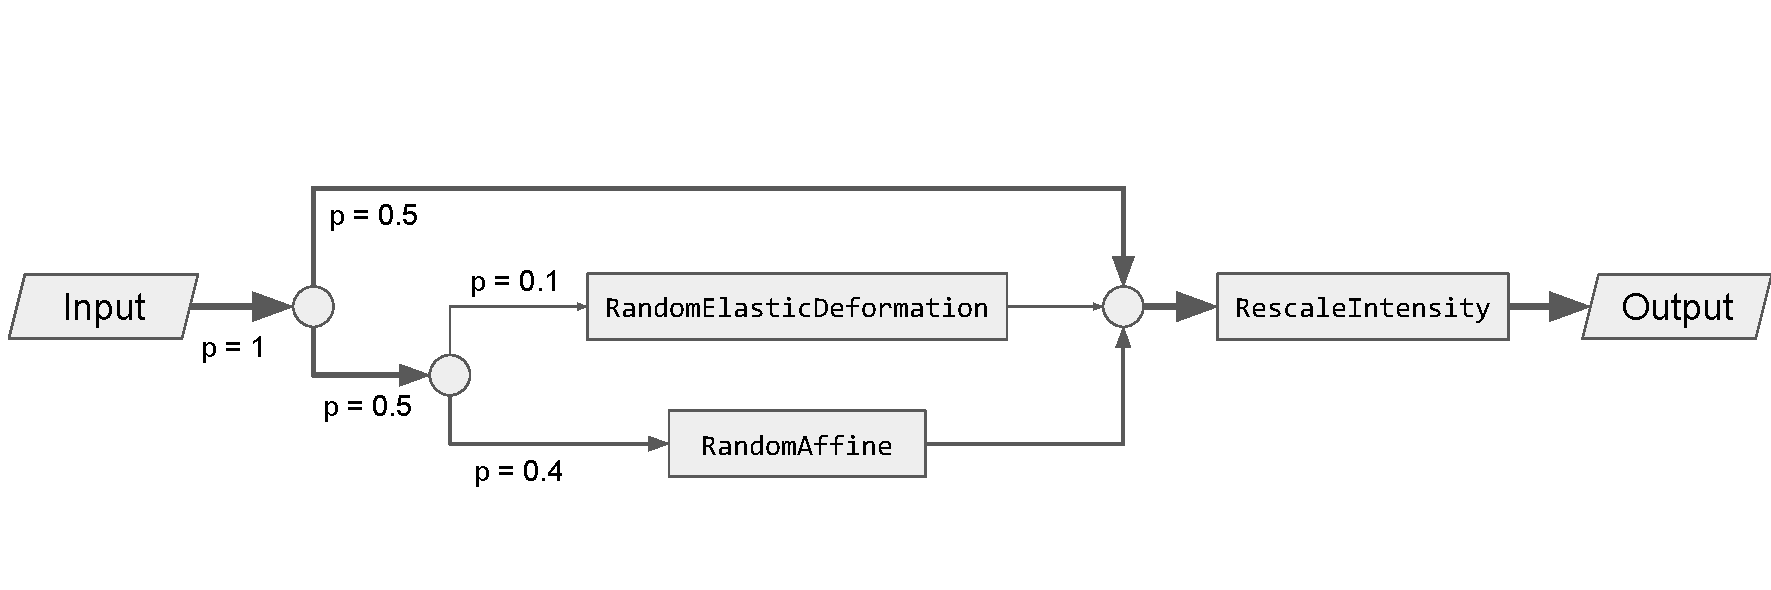
\includegraphics[%
        width=\linewidth,
        trim = {0 1.5cm 0 3cm},
        clip
    ]{diagram_composition}
    \caption{%
        Graph representation of the composed transform
        described in \cref{sec:composability}.
    }
    \label{fig:dag}
\end{figure}

\begin{minted}[
    % mathescape,
    % linenos,
    % numbersep=5pt,
    gobble=2,
    frame=lines,
    framesep=2mm
    ]{python}
  import torchio as tio
  spatial_transforms = {
      tio.RandomElasticDeformation(): 0.2,
      tio.RandomAffine(): 0.8,
  }
  transform = tio.Compose([
      tio.OneOf(spatial_transforms, p=0.5),
      tio.RescaleIntensity((0, 1)),
  ])
\end{minted}


\texttt{Compose} and \texttt{OneOf} are implemented as TorchIO
transforms.


\subsubsection{Extensibility}

The \texttt{Lambda} transform can be passed an arbitrary callable object, which
allows the user to augment the library with custom transforms without having
a deep understanding of the underlying code.


Additionally, more complex transforms can be developed.
%
For example, we implemented a TorchIO transform to simulate brain resection
cavities from preoperative MR images within a self-supervised learning
pipeline~\cite{perez-garcia_simulation_2020}.
%
The \texttt{RandomLabelsToImage} transform may be used to simulate an image from
a tissue segmentation.
%
It can be composed with \texttt{RandomAnisotropy} to train neural networks
agnostic to image contrast and
resolution \cite{billot_learning_2020, billot_partial_2020,iglesias_joint_2020}.


\subsubsection{Reproducibility and traceability}

To promote open science principles, we designed TorchIO to support experiment
reproducibility and traceability.


All transforms support receiving Python primitives as arguments,
which makes TorchIO suitable to be used with a configuration file associated to
a specific experiment.


A history of all applied transforms and their computed
random parameters is saved in the transform output so that the path in the
\ac{DAG} and the parameters used can be traced and reproduced.
%
Furthermore, the \texttt{Subject} class includes a method to compose the
transforms history into a single transform that may be used to reproduce the
exact result (\cref{sec:composability}).


\subsubsection{Invertibility}

Inverting transforms is especially useful in scenarios where one needs to
apply some transformation, infer a segmentation on the transformed data and
then apply the inverse transformation to bring the inference into the original image space.
%
The \texttt{Subject} class includes a method to invert the transformations applied.
%
It does this by first inverting all transforms that are invertible, discarding the ones that are not.
%
Then, it composes the invertible transforms into a single transform.


Transforms invertibility is most commonly applied to
test-time augmentation \cite{moshkov_test-time_2020}
or estimation of aleatoric uncertainty \cite{wang_aleatoric_2019}
in the context of image segmentation.